\documentclass[a4paper,12pt]{article}%twoside
\usepackage{amsfonts, amsmath, amssymb, bm, color, fancyhdr, graphicx, lastpage, listings, natbib, relsize, titling}
\usepackage{hyperref}
\hypersetup{pdftex,colorlinks=true,allcolors=blue}
\usepackage{hypcap}
\usepackage[left=2.5cm,right=2cm]{geometry}
\definecolor{listinggray}{gray}{0.9}
\definecolor{lbcolor}{rgb}{0.9,0.9,0.9}
\usepackage{caption}
\DeclareCaptionFont{black}{\color{black}}
\DeclareCaptionFormat{listing}{\colorbox{\color{listinggray}}{\parbox{0.988\textwidth}{#1#2#3}}}
\captionsetup[lstlisting]{format=listing,labelfont=white,textfont=white}
\lstset{
backgroundcolor=\color{lbcolor},
    tabsize=4,    
%   rulecolor=,
    language=[GNU]C++,
        basicstyle=\scriptsize,
        breakatwhitespace,
        upquote=true,
        aboveskip={1.5\baselineskip},
        columns=fixed,
        showstringspaces=false,
        extendedchars=false,
        breaklines=true,
        prebreak = \raisebox{0ex}[0ex][0ex]{\ensuremath{\hookleftarrow}},
        frame=single,
        numbers=left,
        showtabs=false,
        showspaces=false,
        showstringspaces=false,
        identifierstyle=\ttfamily,
        keywordstyle=\color[rgb]{0,0,1},
        commentstyle=\color[rgb]{0.026,0.112,0.095},
        stringstyle=\color[rgb]{0.627,0.126,0.941},
        numberstyle=\color[rgb]{0.205, 0.142, 0.73},
%      \lstdefinestyle{C++}{language=C++,style=numbers}’.
}
\lstset{
  backgroundcolor=\color{lbcolor},
  breaklines=true,
  %literate={\_}{}{0\discretionary{\_}{}{\_}}%
  tabsize=4,
  language=C++,
  captionpos=t,
  tabsize=3,
  frame=lines,
  numbers=left,
  numberstyle=\tiny,
  numbersep=5pt,
  showstringspaces=false,
  basicstyle=\footnotesize,
%  identifierstyle=\color{magenta},
  keywordstyle=\color[rgb]{0,0,1},
  commentstyle=\color[rgb]{0,0.6,0},
  stringstyle=\color{red}
  }
 
\newcommand\CC{C\nolinebreak[4]\hspace{-.05em}\raisebox{.4ex}{\relsize{-3}{\textbf{++}}}}

%\fancyhead[LE,RO]{\thepage}
\pagestyle{fancy}
%\fancyhead{}% Remove all header contents
\textheight 24cm
\voffset -0.25cm
\footskip 3.5cm
\setlength{\parindent}{0pt}

\makeatletter
%\renewcommand{\headrulewidth}{0pt}% Remove header rule
\renewcommand{\thefootnote}{\roman{footnote}}	

\renewcommand\section{\@startsection{section}{2}{\z@}%
                                     {-3.25ex\@plus -1ex \@minus -.2ex}%
                                     {1.5ex \@plus .2ex}%
                                     {\normalfont\large\bfseries}}% from \large
\renewcommand\subsection{\@startsection{subsection}{2}{\z@}%
                                     {-3.25ex\@plus -1ex \@minus -.2ex}%
                                     {1.5ex \@plus .2ex}%
                                     {\normalfont\bfseries}}
\renewcommand\subsubsection{\@startsection{subsection}{2}{\z@}%
                                     {-3.25ex\@plus -1ex \@minus -.2ex}%
                                     {1.5ex \@plus .2ex}%
                                     {\normalfont\bfseries\itshape}}% from \large                                                                        

% we use \prefix@<level> only if it is defined
\renewcommand{\@seccntformat}[1]{%
  \ifcsname prefix@#1\endcsname
    \csname prefix@#1\endcsname
  \else
    \csname the#1\endcsname\quad
  \fi}
% define \prefix@section
%\newcommand\prefix@section{Section \thesection: }
\newcommand\prefix@section{}

\renewcommand{\@seccntformat}[1]{%
  \ifcsname prefix@#1\endcsname
    \csname prefix@#1\endcsname
  \else
    \csname the#1\endcsname\quad
  \fi}
% define \prefix@section
%\newcommand\prefix@section{Section \thesection: }
\newcommand\prefix@subsection{}

\renewcommand{\@seccntformat}[1]{%
  \ifcsname prefix@#1\endcsname
    \csname prefix@#1\endcsname
  \else
    \csname the#1\endcsname\quad
  \fi}
% define \prefix@section
%\newcommand\prefix@section{Section \thesection: }
\newcommand\prefix@subsubsection{}

\renewcommand{\baselinestretch}{1.15} 

\pretitle{\noindent\Large\bfseries}
\posttitle{\\}
\preauthor{\itshape}
\postauthor{\\}
\pretitle{\begin{center}\Large\bfseries}
\posttitle{\end{center}\\}
\preauthor{\begin{center}\normalsize}
\postauthor{\end{center}\\}
\predate{\begin{center}\itshape}
\postdate{\end{center}\\}
\setlength{\droptitle}{-1.25 in}
\lhead{PiE $\CC$ Final Assignment}
\rhead{Duc Nguyen \quad \thepage\ / \pageref{LastPage}}
\title{PiE $\CC$ Final Assignment}
%\date{\vspace{-5ex}}
\author{Name: Duc Nguyen, \\student number: s1630512\thanks{Email address for 
correspondence: nguyenmanhduc@student.utwente.nl or ngmaduc@gmail.com}}

\begin{document}
\clearpage\maketitle
\thispagestyle{empty}
\pagestyle{fancy}
\newpage
%\maketitle
\section{Exercise 1}
\subsection{Question 1.1}
Write a $\CC$ program to compute the first $N$ prime numbers, where $N$ is given by the user. Use dynamic arrays to store the primes and use this information in the mod test. 
\subsubsection{Answer.}
Three functions are used for this question including $\lstinline{bruteForce, modTest}$ and 
$\lstinline{print_primes}$ for searching prime numbers and printing out the result in console. Passing by reference are chosen to avoid unnecessary copy of variables.
\begin{lstlisting}
std::vector <unsigned long int> bruteForce (int &n);
std::vector <unsigned long int> modTest (int &n);
void print_primes (int &n, const std::vector <unsigned long int>& primes);
\end{lstlisting}
The method chosen to create dynamic arrays to store the primes is $\lstinline{std::vector}$. The range $[0, 2147483647]$ of  $\lstinline{unsigned long int}$ fits to the scope of the question. The idea of $\lstinline{bruteForce}$,\linebreak $\lstinline{modTestDiv}$ are shown in the following code snippets.
\begin{lstlisting}[title = $\lstinline{bruteForce}$]
       primes.push_back(2);
        unsigned long int c;//need to be the type of primes for mode test
        int count = 1;
        for (int count = 1; count < n; ){//counter from 1; "2" included before
            for (c = 2; c < num; c++){
                if (num % c == 0) {//mod test from 2 to n
                    break;	
                }    
            }
            if (c == num) {//to this point means no divisor up to n, Prime!
                primes.push_back(num);//push to result vector of Prime
                count++;//increase counter   
            }
            num++;  
        }
\end{lstlisting}

\begin{lstlisting}[title = $\lstinline{modTestDiv}$]
        primes.push_back(2);  
        for (int count = 1; count < n; ) {//counter from 1; "2" included before 
            bool isPrime = true;
            for (int i = 0; i < primes.size(); i++){
                if (num % primes[i] ==0) {//non-primes  are products of primes
                  isPrime = false;
                  break;
                }    
            }
            if (isPrime == true) {
                primes.push_back(num);
                count++;//increase counter
            }
            num++;
        }
\end{lstlisting}
\subsection{Question 1.2}
Write to the screen a list of the first 10000 primes in the format below; where $p(n)$ is the
$n^{th}$ prime number. Report only the last five lines. Comment on the behaviour of the ratio $n * ln(p(n))/p(n)$ as n gets large.
\subsubsection{Answer.}
The $\lstinline{void print_ratio (int &n, const std::vector <unsigned long int>& primes)}$ and  prime number search functions together generate the required ratio. As $n$ gets large, the ratio tends to converge to 1. Until $10^5-th$ prime number, the ratio is 1.103.\\\\
The last five lines are and the $\lstinline{print_ratio}$ are listed below:
\begin{lstlisting}
9996     :       104707  :       1.10348856177824
9997     :       104711  :       1.10356044403989
9998     :       104717  :       1.10361306655082
9999     :       104723  :       1.10366568381267
10000    :       104729  :       1.10371829582629
\end{lstlisting}

\begin{lstlisting}[title = $\lstinline{print_ratio}$]
void print_ratio (int &n, const std::vector <unsigned long int>& primes){
    std::cout << "n\t:\t p(n)\t:\t n*ln( p(n) )/p(n) " << std::endl;
    for (int i = primes.size; i < primes.size(); i++) {
        std::cout << i+1 << "\t:\t" << primes[i] <<"\t:\t" 
            <<std::fixed << std::setprecision(14) << 
                double((i+1)*log(primes[i])/primes[i])<< std::endl;
        }//set precision used for increase decimal displayed
}
\end{lstlisting}
\subsection{Question 1.3}
Based on question 2, give an estimate of the $10^6-th$ prime number.
\subsubsection{Answer.}
We use 1.1 for the value of the ratio with $n=10^6$:
$$10^6 * ln(p(10^6))/p(10^6) \approx 1.1 $$
Using Wolfram Alpha to solve this equation, the estimate of the $10^6-th$ prime number is:
$$p(10^6) \approx 15022800$$
\subsection{Question 1.4}
Instead of writing to the screen, write to a file (on disk) a list containing just the prime
numbers. Print eight numbers per line, such that all numbers have the same space.
\subsubsection{Answer.}
The $\lstinline{primes_to_file}$ function for writing to a file (on disk) with eight numbers per line is shown below: 
\begin{lstlisting}[title = $\lstinline{primes_to_file}$]
void primes_to_file (int &n, const std::vector <unsigned long int>& primes,
        const std::string& fileName){
        if(n >= 1){
            std::ofstream fileOut;
            fileOut.open(fileName);
            for (int i = 0; i < primes.size(); i++) {
                fileOut << primes[i] << "\t";
                if ((i+1) % 8 == 0) {//Print eight numbers per line
                    fileOut<<std::endl;
                }	
            }
        }
        else{
            std::cerr << "Invalid Input" << std::endl;
        }
}
\end{lstlisting}
\subsection{Question 1.5}
Time your code for $N = 10^3; 10^4; 10^5$ and $10^6$. Make a log-log plot of run-time against $N$ for both codes. What can we say from the log-log plot? Do this analysis for brute force and suggested speed up and comment on the results.
\subsubsection{Answer.}
Figure \eqref{fig1} is the log-log plot of run-time against $N$ showing that within the range of $N$ the linear relationship of logarithmic values of run-time and $N$ which also mean the running time is propotional to $N$ to the power of the slope of the straight line of the log-log graph. The search function $\lstinline{modTestDiv}$ is faster than $\lstinline{bruteForce}$. However, the $\lstinline{bruteForce}$ can be simply modified to $\lstinline{bruteForceM}$ which results in faster running time. The only modification is instead of performing mod test from 2 to $n$ for each number $n$, we only do mod test from 2 to square root of $n$, because number $n$ is not a prime number means that it always has a divisor less than or equal square root of $n$. Otherwise, the number $n$ is a prime number. Measurement of running time is recored by using $\lstinline{std::chrono::time_point<std::chrono::system_clock>}$. The running times are then saved to a file for further processing. All the codes are measured with the function $\lstinline{rtime_to_file}$. Code snippets for  $\lstinline{rtime_to_file}$ and $\lstinline{bruteForceM}$  are shown below:
\begin{figure}[h]
\centering
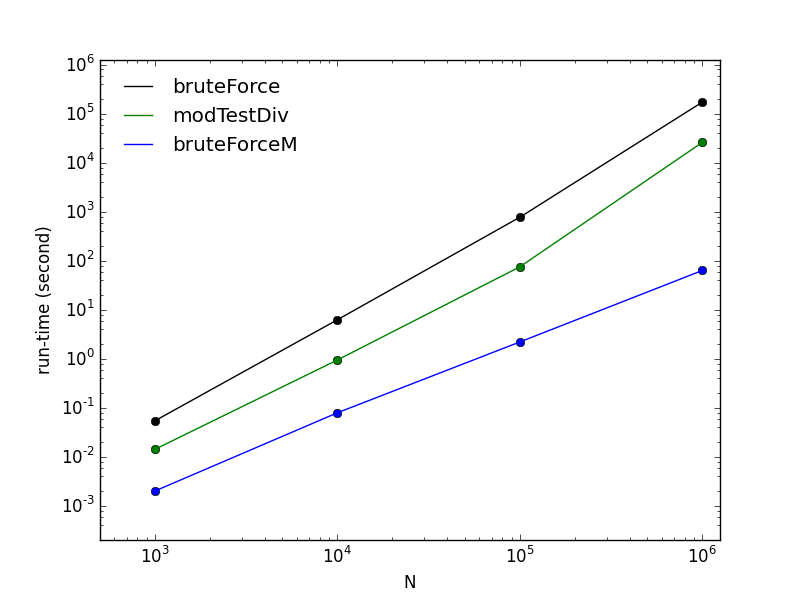
\includegraphics[width=0.8\linewidth, height=0.5\linewidth]{rt-vs-n.png}
\caption{log-log plot of run-time against $N$}
\label{fig1}
\end{figure}
\begin{lstlisting}[title = $\lstinline{rtime_to_file}$]
void rtime_to_file (const std::string& fileName, 
    std::function<std::vector <unsigned long int>(double &n)> &f){    
 	...
    for (int i = 0; i < v.size(); i++) {
        std::chrono::time_point<std::chrono::system_clock> start, end;
        start = std::chrono::system_clock::now();
        std::vector<unsigned long int> primes = f(v[i]);//only measure this function
        end = std::chrono::system_clock::now();
        std::chrono::duration<double> elapsed_seconds = end-start;
 	...    
    }
}
\end{lstlisting}
\begin{lstlisting}[title = $\lstinline{bruteForceM}$]
for (int count = 2; count <= n; ){//counter from 1; "2" included before
            for (c = 2; c <= sqrt(num); c++){//non prime has divisor lt sqrt
                ...
            }
            if (c > sqrt(num)) {//to this point no divisor up to n, Prime!
                ...
            }
            num++;  
        }
\end{lstlisting}
\subsection{Question 1.6}
More efficient ways of computing prime numbers exist. Find and implement one and report
the analysis of part 5 for this algorithm. Comment on the results.
\subsubsection{Answer.}
Sieve of Eratosthenes is used for illustrating an efficient way to search for prime numbers.
The log-log plot of run-time against $N$ is shown in Figure \eqref{fig2}.
\begin{figure}[h!]
\centering
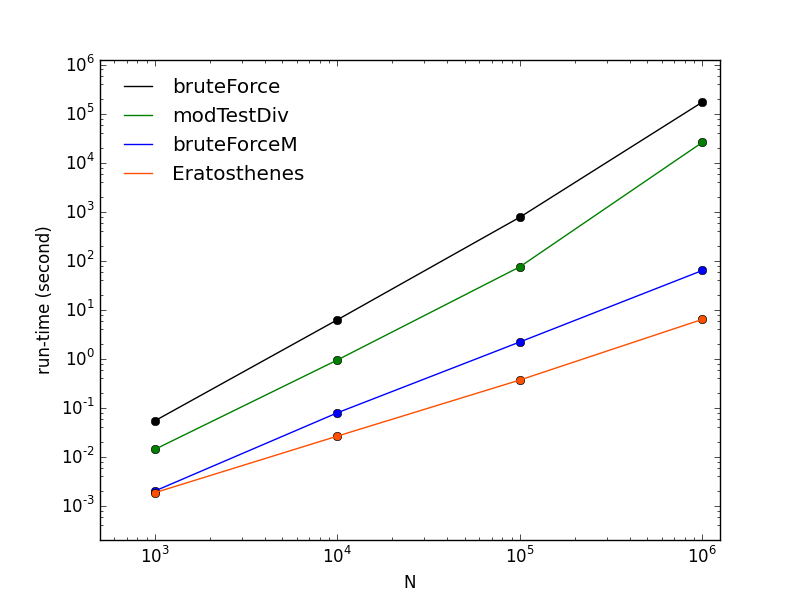
\includegraphics[width=0.8\linewidth, height=0.5\linewidth]{rt-vs-n-eratos.png}
\caption{log-log plot of run-time against $N$}
\label{fig2}
\end{figure}\\
The idea is just to mark all the number in the range of interest as prime then update the mark as non-prime if a number is the multiplication of the previous primes. It illustrate the fundamental property of prime number that any non-prime number can be represented by a multiplication of prime numbers. The code snippet implementing Sieve of Eratosthenes is shown below. The Sieve of Eratosthenes requires the largest number to be found as an input. We can use the ratio from Question 1.3 or Rosser's theorem which states that $p(n) < n * log(n*log(n))$. For searching large prime numbers, the linear relationship will not be held. Further study on complexity of algorithm showing that is beyond the scope of this report. However, a simple test shows that for only 7 digits prime number, high complexity method like $\lstinline{bruteForce}$ already takes the order of days. Therefore, it should not be used for finding large prime numbers. 
\begin{lstlisting}[title = $\lstinline{Eratosthenes}$]
	unsigned long int max = n * std::log(n*std::log(n)); //Rosser's theorem
    for (unsigned long int p=2; p < max; p++){ // for all elements in array
        if (primes.size() > n-1){//keep track first n prime only, vector count from 0
            break;
        }
        else if(isPrime[p] == true){ // it is not multiple of any other prime
            primes.push_back(p);
        }
        // mark all multiples of prime selected above as non primes
        int c=2;
        int mul = p * c;
        while(mul <= max){
            isPrime[mul] = false;
            c++;
            mul = p*c;
        }        
    }
\end{lstlisting}
\section{Exercise 2}
\subsection{Question 2.1}
Read a string input from the terminal (which is assumed to be in RPN). Interpret the string
correctly and output the result to the screen.
Your Reverse Polish Notation calculator should be able to do add, subtract, multiply and
divide integers.
\subsubsection{Answer.}
Three functions are used to build an RPN for integers: $\lstinline{RPN}$ is used for performing arithmethic operation while $\lstinline{parserPostFix}$ and $\lstinline{getFSMCol}$ are used to deal with multi-digit and negative integers.
\begin{lstlisting}
double RPN (const std::vector<std::string>& expr);
std::vector<std::string> parserPostFix(std::string& postfix);
int getFSMCol(char& currentChar);
\end{lstlisting}
The main idea is to parse $\lstinline{std::string& postfix}$ to a $\lstinline{std::vector<std::string>}$ then perform RPN evaluator. The algorithm for RPN evaluator used in this code is described in programming reference \cite[]{roberts2013}.
Parsing function $\lstinline{parserPostFix}$ is done by using a Finite State Machine (listed below) to keep track of keyboard strokes.  It will recognize the consecutive keystrokes to combine keystrokes as multi-digit or negavtive numbers then store to vector elements as a string. RPN evaluator will then convert those string to integer before implement its algorithm. 
\begin{lstlisting}
std::array <std::array<int,5>, 5> stateTable= 
{{{0, INTEGER,  NEGATIVE, OPERATOR, SPACE},
  {INTEGER,  INTEGER,  RESTART,  RESTART,   RESTART},
  {NEGATIVE, INTEGER,  RESTART,  RESTART,   RESTART},
  {OPERATOR,  RESTART, RESTART,  RESTART,   RESTART},
  {SPACE,     RESTART, RESTART,  RESTART,   RESTART}}};
\end{lstlisting}
\begin{lstlisting}
if(currentState == RESTART){
            if(currentToken != " "){
                tokens.push_back(currentToken);//push to new cell
            }
            currentToken = "";
        }
        else{
            //recording multi digit and negative until next RESTART
            currentToken += currentChar;
            ++i;
        }
\end{lstlisting}
The first column can be undestood as first key stroke and the second column can be understood as second keystroke. The highlight here is whenever the state is RESTART, new element in vector is ready while if the state is not RESTART during several keystrokes like in the case of multi-digit or negavtive numbers, it will continue to store in the current vector element.
\subsection{Question 2.2}
Extend your code such that it reads the input line-by-line from a file. Each newline marks
the end of each calculation. Write out the result of each line of the calculation and your
program should abort when it detects an `end of file' condition.
\subsubsection{Answer.}
Function $\lstinline{inputToPostfix}$ with the powerful $\lstinline{std::getline(fileIn,line)}$ check will produce a \linebreak  $\lstinline{std::vector<std::string>postfix}$ with elements corresponding to RPN of each line. Run a simple loop through this vector and do the same as Question 2.1 will write results on console.
\begin{lstlisting}[title = $\lstinline{inputToPostfix}$]
std::vector<std::string> inputToPostfix (const std::string& fileName){
    std::vector<std::string> postfix;
    std::ifstream fileIn(fileName);
    std::string line;
    while (std::getline(fileIn , line)){
        postfix.push_back(line);
    }
    return postfix;
}
\end{lstlisting}
\section{Exercise 3}
\subsection{Question 3.1}
Use any algorithm to compute the shortest distance between every set of cities and write this information to disk with the route as a list of cities.
\subsubsection{Answer.}
The question ask for the shortest distance between every set of cities thus Floyd-Warshall’s algorithm which is well-known for solving to solve the All-Pairs-Shortest-Path problem is chosen. This report will try to cover key points of the algorithm as well as explain how to implement it it $\CC$. The details of Floyd-Warshall’s algorithm used for the code in this exercise is described in Graph Theory reference. \cite[]{ray2013}\\

The input file given is very suitable for the algorithm because it is already in the form of adjacency matrix (distance matrix) which give all information about the cities and how they are connected. They are also known as nodes and edges' length in graph theory. The distance matrix $d$ is stored by 2-D vector $\lstinline{std::vector<std::vector<int>> d}$. To reconstruct the shortest path, we also need a node sequence matrix $s$ which is stored by a 2-D $\lstinline{std::vector<std::vector<int>> s}$. All the elements of node sequence matrix $s$ which means that initially the shortest path is the direct connection from citi $i$ to city $j$. The size of both vector are the square of nodes. The functions $\lstinline{lines_count}$ and $\lstinline{input2vector}$ are used to obtain the number of nodes and create the distance matrix, respectively. We are now ready to implement Floyd-Warshall’s algorithm which is done by the function $\lstinline{WFI}$. 

\begin{lstlisting}
int lines_count (const std::string& fileName);
std::vector<std::vector<int>> input2vector (const std::string& fileName);
void WFI(int &nodes, std::vector<std::vector<int>>& d, 
        std::vector<std::vector<int>>& s);
int main()
{  
	...    
    std::vector<std::vector<int>> s(nodes,std::vector<int>(nodes, 0)); 
    ...
}
\end{lstlisting}

The code snippet for the implementation of  $\lstinline{lines_count}$ and $\lstinline{input2vector}$ are shown below:
\begin{lstlisting}[title = $\lstinline{lines_count}$]
std::ifstream fileIn(fileName);
    int n =0;
    std::string line;
    while (std::getline(fileIn , line)){
        n++;//increase n after each line
    }
\end{lstlisting}

\begin{lstlisting}[title = $\lstinline{input2vector}$]
while (std::getline(fileIn , line)){
        std::vector<int> lineData;
        std::istringstream  lineStream(line);
        int value;
        // Read an integer at a time from the line
        while(lineStream >> value){
            // Add the integers from a line to a 1D vector
            lineData.push_back(value);
        }
        // When all the integers have been read add the 1D array
        // into a 2D array (as one line in the 2D array)
        d.push_back(lineData);
    }
\end{lstlisting}

Floyd-Warshall's algorithm is a recursive algorithm which updates distance matrix $d$ and 
node sequence matrix $s$ in each step. We will run a loop from the first node to the last note. For each iteration, it simply tells whether a city $k$ needs to be included for shortest in the path between city $i$ is city $j$. It will be updated in node sequence matrix $s$ as part of the shortest path and will be permanently as part of the shortest path. The algorithm behave like a greedy algorithm as it prefers more nodes and shortest path. We need the latest status of distance matrix $d$ since it stores the current shortest distance between city $i$ is city $j$. It will only be updated when the current shortest distance from is less than the distance if we include a new node $k$ in the shortest path when we compare the distance in each iteration. There is one small problem with this algorithm that it could not record multiple current shortest distance when it happens to be the equality case for the comparision of the iteration. In this case, I choose to include the one with more nodes in the the shortest paths. The implementaion of Floyd-Warshall’s algorithm is shown below:
\begin{lstlisting}[title = $\lstinline{WFI}$]
	for (int k = 1; k <= nodes; k++){
        for (int i = 1; i <= nodes; i++){
            for (int j = 1; j <= nodes; j++){
                //If the path with two edges is less than the path with one edge
                //node that algorithm is from 1 but vector is from 0
                if(i!=k && j!=k && i!=j){ 
                    if (d[i-1][j-1] >= (d[i-1][k-1] + d[k-1][j-1])){
                        //choose the one with more nodes
                        //Set the cost of the edge to be the lesser cost.
                        d[i-1][j-1] = (d[i-1][k-1] + d[k-1][j-1]);
                        //This ensures proper path reconstruction. 
                        //at this point increase to k+1 to continue algorithm
                        s[i-1][j-1] = k;
                    }
                }
            }  	  
		}
    }        
\end{lstlisting}
Reconstructing the shortest path is like going in a zig-zag in the latest node sequence matrix $s$. The element $s[i][j]$ will tell if the node $k$ is needed to be included in the shortest path. If there is a k, the recuresion will be done for $s[i][k]$ and $s[k][j]$ and it will stops when $k=0$ which is the base case. The function $\lstinline{path_recon_to_file}$ is used for path reconstruction and it is shown as below:
\begin{lstlisting}[title = $\lstinline{path_recon_to_file}$]
void path_recon_to_file(std::ofstream& fileOut1, int& n1,int& n2, 
        std::vector<std::vector<int>>& s){
    int k;
    k = s[n1-1][n2-1];//start and destination, remember to -1 in the index
    if (k != 0){
        path_recon_to_file(fileOut1,n1,k,s);//recursive
        fileOut1 << " - "<< k;//add - to separate new nodes
        path_recon_to_file(fileOut1,k,n2,s);//recursive
    }
} 
\end{lstlisting}
To record all the shortest distance and the shortest path to a file, now all we need to do is to run a loop so that it covers all the pair of nodes then run $\lstinline{WFI}$ and $\lstinline{path_recon_to_file}$. This is be done as shown in the implemetation below:
\begin{lstlisting}
for (int i = 1; i <= d.size(); i++){
            for (int j = i+1; j <= d[i].size(); j++){
                //i,j is correspond to algorithm so start from 1
                //j will start from i+1 because we move to other cities
                fileOut1 << i;
                path_recon_to_file(fileOut1,i,j,s);//path reconstruction  
                fileOut1 << " - " <<j; 
                fileOut1 << "\t\t" << d[i-1][j-1];// print distance
                fileOut1 << std::endl;
            }           
        }
\end{lstlisting}
\subsection{Question 3.2}
Implement Dijkstra's algorithm.
\subsubsection{Answer.}
Following the hint, we try to create a class $\lstinline{City}$ with variables $\lstinline{int distance}$ to the store best distance $\lstinline{bool visited}$ to store whether the city is visit or not and $\lstinline{int cCity}$ to store the connected city. Neccessary procedures such as get and set methods are also included. The class structure is shown as below:
\begin{lstlisting}[title = $\lstinline{City}$]
class City{
    int distance;//store best distance
    bool visited;//visit or not
    int cCity;//other city which it connected to
public:
    City(int distance, bool visited, int cCity){
        set_Values(distance,visited,cCity);//initializer
    };
    void set_Values(int& d, bool& v, int &p);//initializer
    //set methods
    void set_distance(int& d);
    void set_visited(bool& v);
    void set_cCity(int& p);
    //get methods
    int get_distance();
    bool get_visited();
    int get_cCity();
};
\end{lstlisting}
The initialization steps to set visited for all cities to false, set distance for all cities to infinite, set distance for the first city to 0 are done through the code snippets below. We also need the adjacency matrix (distance matrix) which can be done in the same way as described in Floyd-Warshall's implemetation in question 3.1.
\begin{lstlisting}
	int infinity = 1234567;//know from the input file
    //set all to infinity
    std::vector<City> city(nodes,City(infinity,false,0)); 
\end{lstlisting}

\begin{lstlisting}
    //set distance for the first city to 0
    int i_distance = 0;
    bool i_visited = true;
    int i_cCity = 1;
    city[s-1].set_distance(i_distance);
    city[s-1].set_visited(i_visited);
    city[s-1].set_cCity(i_cCity);
\end{lstlisting}
The core of Dijkstra's algorithm to find the shortest route include 4 steps: (1) Find the city with the lowest distance which has not been visited yet; (2) Mark the city as 'visited' ;(3) If the city is the endpoint, stop; (4) Update the connected cities with the distance found. They are implemented in  $\lstinline{Dijkstra}$ fucntion as described below:
\begin{lstlisting}[title = $\lstinline{Dijkstra}$]
// Find shortest route, remember algorithm is from 1, vector is from 0.
    int k = s;//set k is the source point
    do{
        for (int j = 1; j <= nodes; j++){
            if((city[j-1].get_visited() == false) && (d[k-1][j-1]!= INFINITY)){
                if(city[j-1].get_distance() >= city[k-1].get_distance() 
                        + d[k-1][j-1]){
                    //adjacent city with lowest distance to the source
                    //updated from distance matrix
                    int n_distance = city[k-1].get_distance() + d[k-1][j-1];
                    city[j-1].set_distance(n_distance);//best distance so far
                    city[j-1].set_cCity(k);//update connected city for shortest
                }        
            }           
        }
        int min = infinity;
        for (int i = 1; i <= nodes; i++){           
            //two loop looks the same but cannot combined because city[i] should
            //not updated on-the-fly. the second loop needs the first loop done
            if((city[i-1].get_visited() == false) && 
                    (city[i-1].get_distance() < min)){
                min = city[i-1].get_distance();
                k = i;
            }
        }
        bool n_visited = true;
        city[k-1].set_visited(n_visited);//mark as visited
    }
    while (k != t);//if the city is the endpoint, stop, molding completed! 
    return city[t-1].get_distance();    
\end{lstlisting}
The construction of the actual route consists of 5 steps:(1) Start at the last city, (2) Look which connected cities has the lowest distance, (3) Add that one to the route, (4) Consider the city just added to be the last one, (5) Is the last city the begin city? Done!. They are implemented in  $\lstinline{path_recon_to_file}$ fucntion as described below:
\begin{lstlisting}[title = $\lstinline{path_recon_to_file}$]
void path_recon_to_file(std::ofstream& fileOut1, int& s, int& t, int& nodes, std::vector<City>& city){
    std::vector<int> path(nodes); 
    int l = 0;
    fileOut1 << s << " - ";
    for (int v = t; v != s; v = city[v-1].get_cCity()){//start at the last city
        path[l++] = v;//add to route
    }
    for (int i = l; i > 1; i--){//add until the first city i=1
        fileOut1 << path[i-1] << " - ";
    }       
    fileOut1 << t;
}
\end{lstlisting}
\subsection{Question 3.3}
The real TomTom problem.
\subsubsection{Answer.}
This question is out of scope of this report. An attempt using $\lstinline{std::chrono::time_point}$. was made to measure the running time of Floyd-Warshall’s algorithm and Dijkstra's algorithm  With the given input file, the time to listing shortest path for 3 to 50 cites are only $10^{-4}$ to $0.1$ second which does not suffice to comment about which algorithm is better using the codes in this report. From \cite[]{ray2013}, based on complexity analysis, Dijkstra's algorithm is faster because it has lower order of complexity. The speed of Dijkstra's algorithm can be even faster with the use of $\lstinline{heap}$ structure and precomputed data. Further study frotm this report is necessary.
\bibliographystyle{jfm}
% Note the spaces between the initials
\bibliography{ppr}
\end{document}
     